


\tikzset{every picture/.style={line width=0.75pt}} %set default line width to 0.75pt        

\begin{tikzpicture}[x=0.75pt,y=0.75pt,yscale=-1,xscale=1]
%uncomment if require: \path (0,534); %set diagram left start at 0, and has height of 534


% Text Node
\only<1-5,7-8>{\draw (241,27) node [anchor=north west][inner sep=0.75pt]    {$B_{4}$};}
\only<6,9->{\draw (241,27) node [anchor=north west][inner sep=0.75pt]  [color={rgb, 255:red, 255; green, 0; blue, 0 }  ,opacity=1 ]    {$B_{4}$};}
% Text Node
\only<1-3>{\draw (283,59) node [anchor=north west][inner sep=0.75pt]    {$B_{2}$};}
\only<4->{\draw (283,59) node [anchor=north west][inner sep=0.75pt]  [color={rgb, 255:red, 124; green, 216; blue, 23 }  ,opacity=1 ]    {$B_{2}$};}
% Text Node
\only<1-4,8-9>{\draw (323,27) node [anchor=north west][inner sep=0.75pt]    {$B_{3}$};}
\only<5-7,10->{\draw (323,27) node [anchor=north west][inner sep=0.75pt]  [color={rgb, 255:red, 250; green, 153; blue, 3 }  ,opacity=1 ]    {$B_{3}$};}
% Text Node
\only<1-2>{\draw (283,108) node [anchor=north west][inner sep=0.75pt]    {$B_{1}$};}
\only<3->{\draw (283,108) node [anchor=north west][inner sep=0.75pt]  [color={rgb, 255:red, 0; green, 0; blue, 255 }  ,opacity=1 ]    {$B_{1}$};}
% Connection
\draw    (279,57.79) -- (264.57,46.45) ;
\draw [shift={(263,45.21)}, rotate = 38.16] [color={rgb, 255:red, 0; green, 0; blue, 0 }  ][line width=0.75]    (10.93,-3.29) .. controls (6.95,-1.4) and (3.31,-0.3) .. (0,0) .. controls (3.31,0.3) and (6.95,1.4) .. (10.93,3.29)   ;
% Connection
\draw    (305,57.54) -- (318.44,46.72) ;
\draw [shift={(320,45.46)}, rotate = 141.17] [color={rgb, 255:red, 0; green, 0; blue, 0 }  ][line width=0.75]    (10.93,-3.29) .. controls (6.95,-1.4) and (3.31,-0.3) .. (0,0) .. controls (3.31,0.3) and (6.95,1.4) .. (10.93,3.29)   ;
% Connection
\draw    (292,83) -- (292,104) ;
\draw [shift={(292,81)}, rotate = 90] [color={rgb, 255:red, 0; green, 0; blue, 0 }  ][line width=0.75]    (10.93,-3.29) .. controls (6.95,-1.4) and (3.31,-0.3) .. (0,0) .. controls (3.31,0.3) and (6.95,1.4) .. (10.93,3.29)   ;
% Connection
\draw    (298.5,104) -- (325.61,49.79) ;
\draw [shift={(326.5,48)}, rotate = 116.57] [color={rgb, 255:red, 0; green, 0; blue, 0 }  ][line width=0.75]    (10.93,-3.29) .. controls (6.95,-1.4) and (3.31,-0.3) .. (0,0) .. controls (3.31,0.3) and (6.95,1.4) .. (10.93,3.29)   ;

\onslide<14->{\draw (228,73) node [anchor=north west][inner sep=0.75pt]  [color={rgb, 255:red, 255; green, 0; blue, 0 }  ,opacity=1 ]  {$\hat{G}(B_{4})$};

%Curve Lines [id:da02533473137358766] 
\draw [color={rgb, 255:red, 255; green, 0; blue, 0 }  ,draw opacity=1 ]   (260,24) .. controls (299,48) and (316,61) .. (309,110) ;
%Curve Lines [id:da2150259195395825] 
\draw [color={rgb, 255:red, 255; green, 0; blue, 0 }  ,draw opacity=1 ]   (244,48) .. controls (225,35) and (242,13) .. (260,24) ;
%Curve Lines [id:da46500745717824676] 
\draw [color={rgb, 255:red, 255; green, 0; blue, 0 }  ,draw opacity=1 ]   (244,48) .. controls (284,73) and (282,73) .. (279,107) ;
%Curve Lines [id:da9402495253404746] 
\draw [color={rgb, 255:red, 255; green, 0; blue, 0 }  ,draw opacity=1 ]   (309,110) .. controls (308,134) and (276,145) .. (279,107) ;}

\end{tikzpicture}
